
% Can also go beyond and define dynamical quantum $SU(n,1)$, starting from one-parameter space of complex projective spaces. Works for all hermitian symmetric spaces


%The relations for the adjoint further imply that \begin{eqnarray*}u_{kl}^{+-} &=&\frac{E(l,l-1)}{E(k,k+1)}(u_{k+1,l-1}^{-+})^*,\\  u_{kl}^{++}&=& \frac{E(l,l+1)}{E(k,k+1)}(u_{k+1,l+1}^{--})^* .\end{eqnarray*}


%\begin{eqnarray*} u_{++} &=& \frac{w_+(\rho)^{1/2}}{w_+(\lambda)^{1/2}}u_{--}^*,\\u_{+-}&=& (-1)^{s_q}  \frac{w_-^{1/2}(\rho)}{w_+^{1/2}(\lambda)}u_{-+}^*.  \\ 
%\end{eqnarray*}

%Let us write \[F(k) = |q|^{-1}w_+(k) =  |q|^{-1}\frac{|q|^{x+k+1}+|q|^{-x-k-1}}{|q|^{x+k}+|q|^{-x-k}},\] and further put\[\alpha = \frac{F^{1/2}(\rho-1)}{F^{1/2}(\lambda-1)}u_{--},\qquad \beta = \frac{1}{F^{1/2}(\lambda-1)}u_{-+}.\] Then the unitarity of $(u_{\epsilon,\nu})_{\epsilon,\nu}$ together with \eqref{EqAdju} and \eqref{EqGradu} are equivalent to the commutation relations \begin{equation}\label{EqqCom} \alpha \beta = qF(\rho-1)\beta\alpha \qquad \alpha\beta^* = qF(\lambda)\beta^*\alpha\end{equation} \begin{equation}\label{EqDet} \alpha\alpha^* +F(\lambda)\beta^*\beta = 1,\qquad \alpha^*\alpha+q^{-2}F(\rho-1)^{-1}\beta^*\beta = 1,\end{equation}\begin{equation*} F(\rho-1)^{-1}\alpha\alpha^* +\beta\beta^* = F(\lambda-1)^{-1},\qquad  F(\lambda)\alpha^*\alpha +q^{-2}\beta\beta^* = F(\rho),\end{equation*} \begin{equation}\label{EqGrad} f(\lambda)g(\rho)\alpha =
%\alpha f(\lambda+1)g(\rho+1),\qquad f(\lambda)g(\rho)\beta = \beta f(\lambda+1)g(\rho-1).\end{equation}%layout might be nicer

%These are precisely the commutation relations for the dynamical quantum $SU(2)$-group as in \cite[Definition 2.6]{KoR1}, except that the precise value of $F$ has been changed by a shift in the parameter domain by a complex constant. Clearly, by Theorem \ref{TheoGenRel} the (total) coproduct on $A_x$ also agrees with the one on the dynamical quantum $SU(2)$-group, namely \begin{eqnarray*} \Delta(\alpha) &=& \Delta(1) (\alpha\otimes \alpha - q^{-1}\beta\otimes \beta^*),\\ \Delta(\beta) &=& \Delta(1)(\beta\otimes \alpha^* +\alpha\otimes \beta)\end{eqnarray*} where $\Delta(1) = \sum_{k\in \Z} \rho_k\otimes \lambda_k$.

%Let us write $B_x = B_x(\Gamma)$ for the $*$-algebra generated by a copy of the $*$-algebra $c_b(\Z\times \Z)$ of bounded functions on $\Z\times \Z$ as well as elements $\alpha,\beta$ satisfying the relations \eqref{EqqCom}, \eqref{EqDet} and \eqref{EqGrad}.

% Lemma doesn't work because $\alpha$,$\beta$ not bounded.
%\begin{Lem} There is a one-to-one correspondence between non-degenerate $*$-representations of $A_x$ on Hilbert spaces and unital $^*$-representations of $B_x$ on Hilbert spaces for which the restriction to $c_b(\Z\times \Z)$ is strictly continuous.
%\end{Lem}



\section{The universal C$^*$-algebra of the dynamical quantum $SU(2)$}\label{SecUni}

We assume in the following that $0<q<1$ and $\sigma \in \{-1,+1\}$. We also choose $x>0$.
%We also choose $x\in \lbrack \sqrt{q},1\rbrack$.

Denote $\ctau(y) = y+y^{-1}$ and $w_{\pm}(y) = \frac{\ctau(q^{\pm}y)}{\ctau(y)}$. Denote $\sigma_+ = 1$ and $\sigma_- = -\sigma$. Let $\Lambda_x = xq^{\Z}$, and let $B$ be the $^*$-algebra of finite support functions on $\Lambda_x\times \Lambda_x$, whose Dirac functions we write as $\delta_{(y,z)}=\UnitC{y}{z}$. Let $A_x$ be the $^*$-algebra generated by a copy of $B$ and elements \[(u_{\epsilon,\nu})_{y,z}\] for $\epsilon,\nu\in \{-1,1\}=\{-,+\}$ and $y,z\in \Lambda_x$ with defining relations \begin{eqnarray*} \sum_{\mu\in \{\pm\}} (u_{\mu,\epsilon})_{q^{-\mu}w,y}^* (u_{\mu,\nu})_{q^{-\mu}w,z}&=& \delta_{y,z} \delta_{\epsilon,\nu} \UnitC{w}{q^{\epsilon}y},\\ \sum_{\mu\in \{\pm\}} (u_{\epsilon,\mu})_{y,w} (u_{\nu,\mu})_{z,w}^* &=& \delta_{\epsilon,\nu}\delta_{y,z} \UnitC{y}{w} \\ (u_{\epsilon,\nu})_{y,z}^* &=& \frac{\sigma_{\nu}w_{\nu}(z)^{1/2}}{\sigma_{\epsilon}w_{\epsilon}(y)^{1/2}} (u_{-\epsilon,-\nu})_{q^{\epsilon}y,q^{\nu}z}.\end{eqnarray*} The element $(u_{\epsilon,\nu})_{y,z}$ lives inside the component $\Gr{(A_x)}{y}{q^{\epsilon}y}{z}{q^{\nu}z}$.

Consider $M(A_x)$, the multiplier algebra of $A_x$. For a function $f$ on $\Lambda_x\times \Lambda_x$, write $f(\lambda,\rho) = \sum_{y,z} f(y,z)\UnitC{y}{z} \in M(A_x)$. Similarly, for a function $f$ on $\Lambda_x$ we write $f(\lambda) = \sum_{y,z} f(y)\UnitC{y}{z}$ and $f(\rho) = \sum_{y,z}f(z)\UnitC{y}{z}$. We then write for example $f(q\lambda,\rho)$ for the element corresponding to the function $(y,z)\mapsto f(qy,z)$.

We can further form in $M(A_x)$ the elements $u_{\epsilon,\nu} = \sum_{y,z} (u_{\epsilon,\nu})_{y,z}$. Then $u=(u_{\epsilon,\nu})$ is a unitary 2$\times$2 matrix. Moreover, \begin{equation}\label{EqAdju}u_{\epsilon,\nu}^* = u_{-\epsilon,-\nu}\frac{ \sigma_{\nu}w_{\nu}^{1/2}(\rho)}{\sigma_{\epsilon}w_{\epsilon}^{1/2}(\lambda)} ,\end{equation} where $w_{\pm}^{1/2}(y) = w_{\pm}(y)^{1/2}$.  We then have the following commutation relations between functions on $\Lambda_x\times \Lambda_x$ and the entries of $u$: \begin{equation}\label{EqGradu} f(\lambda,\rho)u_{\epsilon,\nu} = u_{\epsilon,\nu}f(q^{-\epsilon}\lambda,q^{-\nu}\rho).\end{equation}

In the following, we write $u_{--}=\alpha, u_{-+}= \beta, u_{+-}=\gamma,u_{++}=\delta$. We then have the following relations.


\[\left\{\begin{array}{lllllll} \alpha\alpha^* + \beta\beta^* &=& 1 &&  \gamma\gamma^* + \delta\delta^* &=& 1,\\ \alpha^*\alpha+ \gamma^*\gamma &=&1,&&\beta^*\beta+ \delta^*\delta &=& 1,\\ \\ \alpha \gamma^* = -\beta \delta^*, &&&& \alpha^*\beta = -\gamma^*\delta, \end{array}\right.\]

\[ \delta =  \frac{w_+^{1/2}(\rho)}{w_+^{1/2}(\lambda)}\alpha^*, \quad \gamma=  -\sigma \frac{w_{-}^{1/2}(\rho)}{w_+^{1/2}(\lambda)}\beta^*,\quad  \beta = -\sigma \frac{w_+^{1/2}(\lambda)}{w_{-}^{1/2}(\rho)}\gamma^*, \quad  \alpha = \delta^* \frac{w_+^{1/2}(\lambda)}{w_+^{1/2}(\rho)}.\]


We wish to classify the irreducible $^*$-representations of $A_x$. We will need an auxiliary notion.

%The parametrisation will hinge on the classification of what we call irreducible $$-adapted sets, which we will now discuss.

%\subsection{Irreducible $c$-sets}

\begin{Def}\label{DefAdapt} Let $c\in\R$. For $\epsilon \in \{\pm\}$, an element $y>0$ will be called \emph{$c_{\epsilon}$-adapted} if \begin{equation}\label{EqAd+} c \leq \ctau(q^{-\epsilon}y),\end{equation} and \emph{strictly} $c_{\epsilon}$-adapted if this holds strictly. It is called \emph{$c$-adapted} if it is both $c_+$- and $c_-$-adapted. 

A subset $Z$ of $\R^+_0$ is called a \emph{$c$-set} if the following conditions hold: \begin{itemize} 
\item[$\bullet$] $Z$ is not empty.
\item[$\bullet$] $Z$ consists of $c$-adapted points.
\item[$\bullet$] If $y\in Z$ is strictly $c_{\epsilon}$-adapted, then $q^{-2\epsilon}y$ is in $Z$.
\end{itemize}
%An $(x,c)$-set $Z$ is called \emph{even} (resp.~ \emph{odd}) if $Z\subseteq q^{2\Z}$ (resp.~ $Z\subseteq q^{2\Z+1}$).
A $c$-set is called \emph{irreducible} if it can not be written as the union of two disjoint $c$-sets.
\end{Def}

We will classify irreducible $c$-sets. For $y>0$, we write $T_y = yq^{1+2\Z}$, $T_y^+ = yq^{1+2\N}$ and $T_y^{-} = yq^{-1-2\N}$. 

%We use the convention $\N = \{0,1,2,\ldots\}$ and $\N_0=\{1,2,\ldots\}$.

\begin{Prop}\label{PropClass1D}

% Picture!
\begin{itemize} The following list exhausts all irreducible $c$-sets.
\item[$\bullet$] $c<2: T_y, y>0$
\item[$\bullet$] $c \geq 2$, $c=\ctau(z)$ with $0 < z\leq 1$:
\begin{itemize}
\item[$\bullet$] $T_y$ for $\frac{q}{z}<qy<\frac{z}{q}$.
\item[$\bullet$] $T_{z}^+$ and $T_{1/z}^-$.
\item[$\bullet$] $\{1\}$ if $z=q$.
\end{itemize}
\end{itemize}
\end{Prop} 
\begin{proof} Elementary.
\end{proof} 

\subsection{Representation theory of $A_x$}

Let us now return to the representation theory of the $^*$-algebra $A_x$.

Let $\pi$ be any (necessarily bounded) non-degenerate $^*$-representation of $A_x$ on a Hilbert space $\Hsp_{\pi}$. Then \[\Hsp_{\pi} = \oplus \Hsp^{y}_{z},\qquad \Hsp^{y}_{z} = \pi(\UnitC{y}{z})\Hsp.\] Write \[H_{\pi} =  \textrm{the (non-closed) linear span of all }\Hsp^{y}_{z}.\] Then $\pi(A_x)H_{\pi} = H_{\pi}$. It follows that one can extend $\pi$ to a map \[\pi: M(A_x) \rightarrow \End_{\adj}(H_{\pi}),\] where $\End_{\adj}(H_{\pi})$ denotes the $^*$-algebra of adjointable operators on the pre-Hilbert space $H_{\pi}$. In particular, the generators $\alpha,\beta,\gamma,\delta$ and their adjoints give rise to (contractive) maps $H_{\pi}\rightarrow H_{\pi}$. 

We have the following easy lemma.

\begin{Lem} There is a one-to-one correspondence between\begin{itemize}\item[$\bullet$] non-degenerate $^*$-representations $(\Hsp_{\pi},\pi)$ of $A_x$ on Hilbert spaces, and 
\item[$\bullet$] $\Lambda_x$-bigraded pre-Hilbert spaces $H_{\pi}$ with norm-complete components and equipped with adjointable maps $\alpha,\beta:H_{\pi}\rightarrow H_{\pi}$ satisfying the commutation relations as in \eqref{EqqCom}, \eqref{EqDet} and \eqref{EqGrad} and with $f(\lambda,\rho)\xi = f(y,z)\xi$ for $f$ a function on $\Lambda_x\times \Lambda_x$ and $\xi\in H^x_y$.
\end{itemize}
\end{Lem}

\begin{Def} The \emph{Casimir} of $A_x$ is defined to be the following element $\Omega\in M(A_x)$, \[\Omega = \ctau(q\lambda/\rho) - \ctau(\lambda)\ctau(\rho/q)\beta^*\beta.\]  
\end{Def}

\begin{Lem} The element $\Omega$ is a self-adjoint central element in $M(A_x)$.
\end{Lem}
\begin{proof}
This follows from a straightforward calculation, cf. \cite[Lemma 3.3]{KoR1}. By self-adjointness, it suffices to check that $\Omega$ commutes with $\delta^*$ and $\beta^*$. The first commutation follows from the skew commutativity relations and the relation $\ctau(q\lambda)\ctau(\rho)\gamma\gamma^* =\ctau(\lambda)\ctau(\rho/q)\beta^*\beta$. The second commutation follows by using the identity \[\beta\beta^* =  \frac{w_+(\rho/q)-w_+(\lambda/q)}{w_+(\rho/q)} + \frac{w_+(\lambda/q)}{w_+(\rho/q)}\beta^*\beta\] and some elementary computations with the $\tau$-function.
\end{proof}

\begin{Cor}\label{CorCas} If $\pi$ is an irreducible $^*$-representation of $A_x$, there exists $c\in \R$ such that $\pi(\Omega)\xi = c\xi$ for all $\xi \in V_{\pi}$. 
\end{Cor} 
\begin{proof} As $\pi(\Omega)$ is bounded when restricted to any $V^y_z$, this follows immediately from a spectral argument. 
\end{proof} 

The following lemma follows from a straightforward computation, using the relations \eqref{EqDet}.

\begin{Lem}\label{LemAmp} Inside $M(A_x)$, we have the following identities:
\begin{eqnarray*}
\alpha^*\alpha &=& \frac{\ctau(q\lambda\rho)+\Omega}{\ctau(\lambda)\ctau(q\rho)}\\
\alpha\alpha^* &=& \frac{\ctau(\lambda\rho/q)+\Omega}{\ctau(\lambda/q)\ctau(\rho)}\\ 
\beta^*\beta &=& \frac{\ctau(q\lambda/\rho)-\Omega}{\ctau(\lambda)\ctau(\rho/q)}\\
\beta\beta^* &=&  \frac{\ctau(\lambda/q\rho)-\Omega}{\ctau(\lambda/q)\ctau(\rho)}.
\end{eqnarray*}
\end{Lem}

Note that the right hand sides are well-defined because of centrality of $\Omega$.

\begin{Cor}\label{CorOneDim} If $\pi$ is an irreducible $^*$-representation of $A_x$ on a Hilbert space $\Hsp_{\pi}$, then $\Hsp^y_z$ is at most one-dimensional for each $y,z\in \Lambda_x$. Moreover, either all $\Hsp^y_z$ with $y/z\in q^{2\Z+1}$ are zero, or all $\Hsp^y_z$ with $y/z\in q^{2\Z}$ are zero. 
\end{Cor} 
\begin{proof} 
Using Corollary \ref{CorCas}, the first assertion follows immediately from \eqref{EqqCom}, the grading relations \eqref{EqGrad} and Lemma \ref{LemAmp}. The second assertion follows immediately from the grading relations \eqref{EqGrad}.
\end{proof}

\begin{Def} Let $(\Hsp_{\pi},\pi)$ be an irreducible $^*$-representation of $A_x$. We call $\pi$ even (resp. odd) if all $\Hsp^y_z$ with $y/z \in q^{2\Z+1}$ (resp.~ $q^{2\Z}$) are zero.
\end{Def} 

%We can hence identity $\Hsp$ as a quotient of $l^2(\Z\times \Z)$. Write the images of the standard basis vectors $e_{m,n}$ of $l^2(\Z\times \Z)$ as $f_{m,n}$. Let us write $F = \{(m,n)\mid f_{m,n}\neq 0\}$.

With the above preliminaries, we can now classify the irreducible $^*$-representations of $A_x$. We first extend the terminology of Definition \ref{DefAdapt}.
% Different order of introducing?


\begin{Def} Fix $c\in \R$. For $\epsilon,\nu\in \{-,+\}$, a couple $(y,z)\in \R_+^2$ is called \emph{$c_{\epsilon,\nu}$-adapted} if the following inequality holds: \begin{equation}\label{EqAd} \ctau(q^{-\epsilon}yz^{\epsilon\nu})+\epsilon\nu c\geq 0.\end{equation} A couple $(y,z)$ is called \emph{strictly} $c_{\epsilon,\nu}$-adapted if this is a strict equality. We call $(y,z)$ \emph{$c$-adapted} if it is $c_{\epsilon,\nu}$-adapted for all $\epsilon,\nu\in \{+,-\}$. 
\end{Def} 

\begin{Def} Fix $c\in \R$. We call a subset $T\subseteq \R_+^2$ a \emph{$c$-set} if the following conditions are satisfied: 
\begin{itemize} 
\item[$\bullet$] $T$ is not empty.
\item[$\bullet$] $T$ consists of $c$-adapted points.
\item[$\bullet$] If $(y,z)\in T$ is strictly $c_{\epsilon,\nu}$-adapted, then $(q^{-\epsilon}y,q^{-\nu}z)$ is in $T$.
\end{itemize}

We say that $T$ \emph{irreducible} if it is not the disjoint union of two $c$-sets.

%Writing $\Z^2_{\even} = \{(k,l)\mid k-l \textrm{ even}\}$ and $\Z^2_{\odd} = \Z^2\setminus \Z^2_{\even}$, we call an $(x,c)$-set even or odd according to whether it lies in $\Z^2_{\even}$ or $\Z^2_{\odd}$.
\end{Def}

\begin{Def} Fix $x>0$. For $\pi$ an irreducible representation of $A_x$, a couple $(y,z)\in \Lambda_x\times \Lambda_x$ is called $\pi$-compatible if $\Hsp^y_z\neq 0$. 

For $c\in \R$, a subset $T\subseteq \Lambda_x\times \Lambda_x$ is called \emph{$(x,c)$-compatible} if there exists an irreducible representation $\pi$ of $A_x$ with $\pi(\Omega) = c$ and $T=\{(y,z)\in \Lambda_x\times \Lambda_x\mid \Hsp^{y}_{z}\neq \{0\}\}$. In this case, we say that $\pi$ is \emph{$T$-adapted}.
\end{Def}

\begin{Prop}\label{PropClassRep} A set $T\subseteq \Lambda_x\times \Lambda_x$ is an irreducible $c$-set if and only if it is an $(x,c)$-compatible set. Moreover, for any $(x,c)$-compatible set $T$ there is exactly one irreducible $^*$-representation $\pi$ of $A_x$, up to unitary equivalence, which is $T$-compatible.
\end{Prop}

\begin{proof} Assume first that $T$ is $(x,c)$-compatible, and let $\pi$ be a $T$-compatible irreducible $^*$-representation of $A_x$. If $(y,z)\in T$, then it follows from Lemma \ref{LemAmp} that $(y,z)$ is $c$-adapted. Moreover, if $(y,z)\in T$ is strictly $c_{\epsilon,\nu}$-adapted, then we have that $\|u_{\epsilon,\nu}\xi\|\neq 0$ for a non-zero $\xi\in \Hsp^y_z$, hence also $\Hsp^{q^{-\epsilon}y}_{q^{-\nu}z}\neq \{0\}$. It follows that $T$ is a $c$-set. Now if $T=T_1\cup T_2$ a disjoint union of $c$-sets, it would follow that $\pi$ restricts to the direct sum of all $\Hsp^y_z$ with $(y,z)\in T_1$, contradicting irreducibility. It follows that $T$ is an irreducible $c$-set.

Conversely, let $T$ be an irreducible $c$-set inside $\Lambda_x\times \Lambda_x$. Put $\Hsp_{\pi} = l^2(T)$ with \begin{eqnarray*} \pi(\alpha) e_{y,z} &=&  \left(\frac{\ctau(qyz)+c}{\ctau(y)\ctau(qz)}\right)^{1/2}e_{qy,qz},\\ \pi(\beta) e_{y,z} &=& \sigma_y\left(\frac{\ctau(qy/z)-c}{\ctau(y)\ctau(z/q)}\right)^{1/2} e_{qy,z/q},\end{eqnarray*} where the right hand side is considered as the zero vector when the scalar factor on the right is zero, and where $\sigma_y = -\sigma$ if $y\in xq^{2\Z+1}$ and $1$ otherwise. Note that the roots on the right hand side are well-defined precisely because $T$ is a $c$-set. 

By direct computation, using the defining commutation relations \eqref{EqqCom} and \eqref{EqDet}, we see that $\pi$ defines a $^*$-representation of $A_x$ with $\pi(\Omega) =c$. Moreover, $\pi$ is irreducible since otherwise, by Corollary \ref{CorOneDim}, $T$ would split as a disjoint union of $(x,c)$-compatible sets. Hence $T$ is an $(x,c)$-compatible set.

Now the formulas for $\pi(\alpha)$ and $\pi(\beta)$ are uniquely determined up to a unimodular gauge factor. As any non-zero $\Hsp^{y}_z$ is cyclic for $\pi$, it follows that these gauge factors are determined by their value at one component. We then easily conclude that $\pi$ is in fact the unique $T$-compatible $^*$-representation, up to unitary equivalence.
\end{proof}

What remains is to classify irreducible $c$-sets for each $c\in \R$. 

\begin{Lem}\label{LemClass2D} A set $T\subseteq \R_+^2$ is an irreducible $c$-set if and only if there exists an irreducible $-c$-set $Z_+\subseteq \R_+$ and an irreducible $c$-set $Z_-\subseteq \R_+$ such that $(y,z)\in T$ if and only if $yz\in Z_+$ and $y/z\in Z_-$.
\end{Lem} 

\begin{proof} It is immediate that $(y,z)\in \R_+^2$ is (strictly) $c_{\epsilon,\nu}$-adapted if and only if $yz^{\epsilon\nu}$ is (strictly) $(-\epsilon\nu c)_{\epsilon}$-adapted. The conclusion of the lemma then follows immediately.
\end{proof}

Combining Proposition \ref{PropClassRep} with Proposition \ref{PropClass1D} and Lemma \ref{LemClass2D}, we thus obtain a concrete description of the spectrum of $A_x$. The following pictures illustrate the form of the spectrum of $A_x$ for the case $q>0$.

\begin{figure}[h]
  \centering
\input{specx0-even.epic}
  \caption{Case $x=0$, even}
\label{figy}
\end{figure}

% Probably in figure below the middle dot at $-t_0$ should be unfilled!
\begin{figure}[h]
  \centering
\input{specx0-odd.epic}
  \caption{Case $x=0$, odd}
\label{figy}
\end{figure}


\begin{figure}[h]
  \centering
\input{specx12-even.epic}
  \caption{Case $x=\frac{1}{2}$, even}
\label{figy}
\end{figure}


\begin{figure}[h]
  \centering
  \input{specx12-odd.epic}
  
  \caption{Case $x=\frac{1}{2}$, odd}
\label{figy}
\end{figure}

% Should be latexed?
%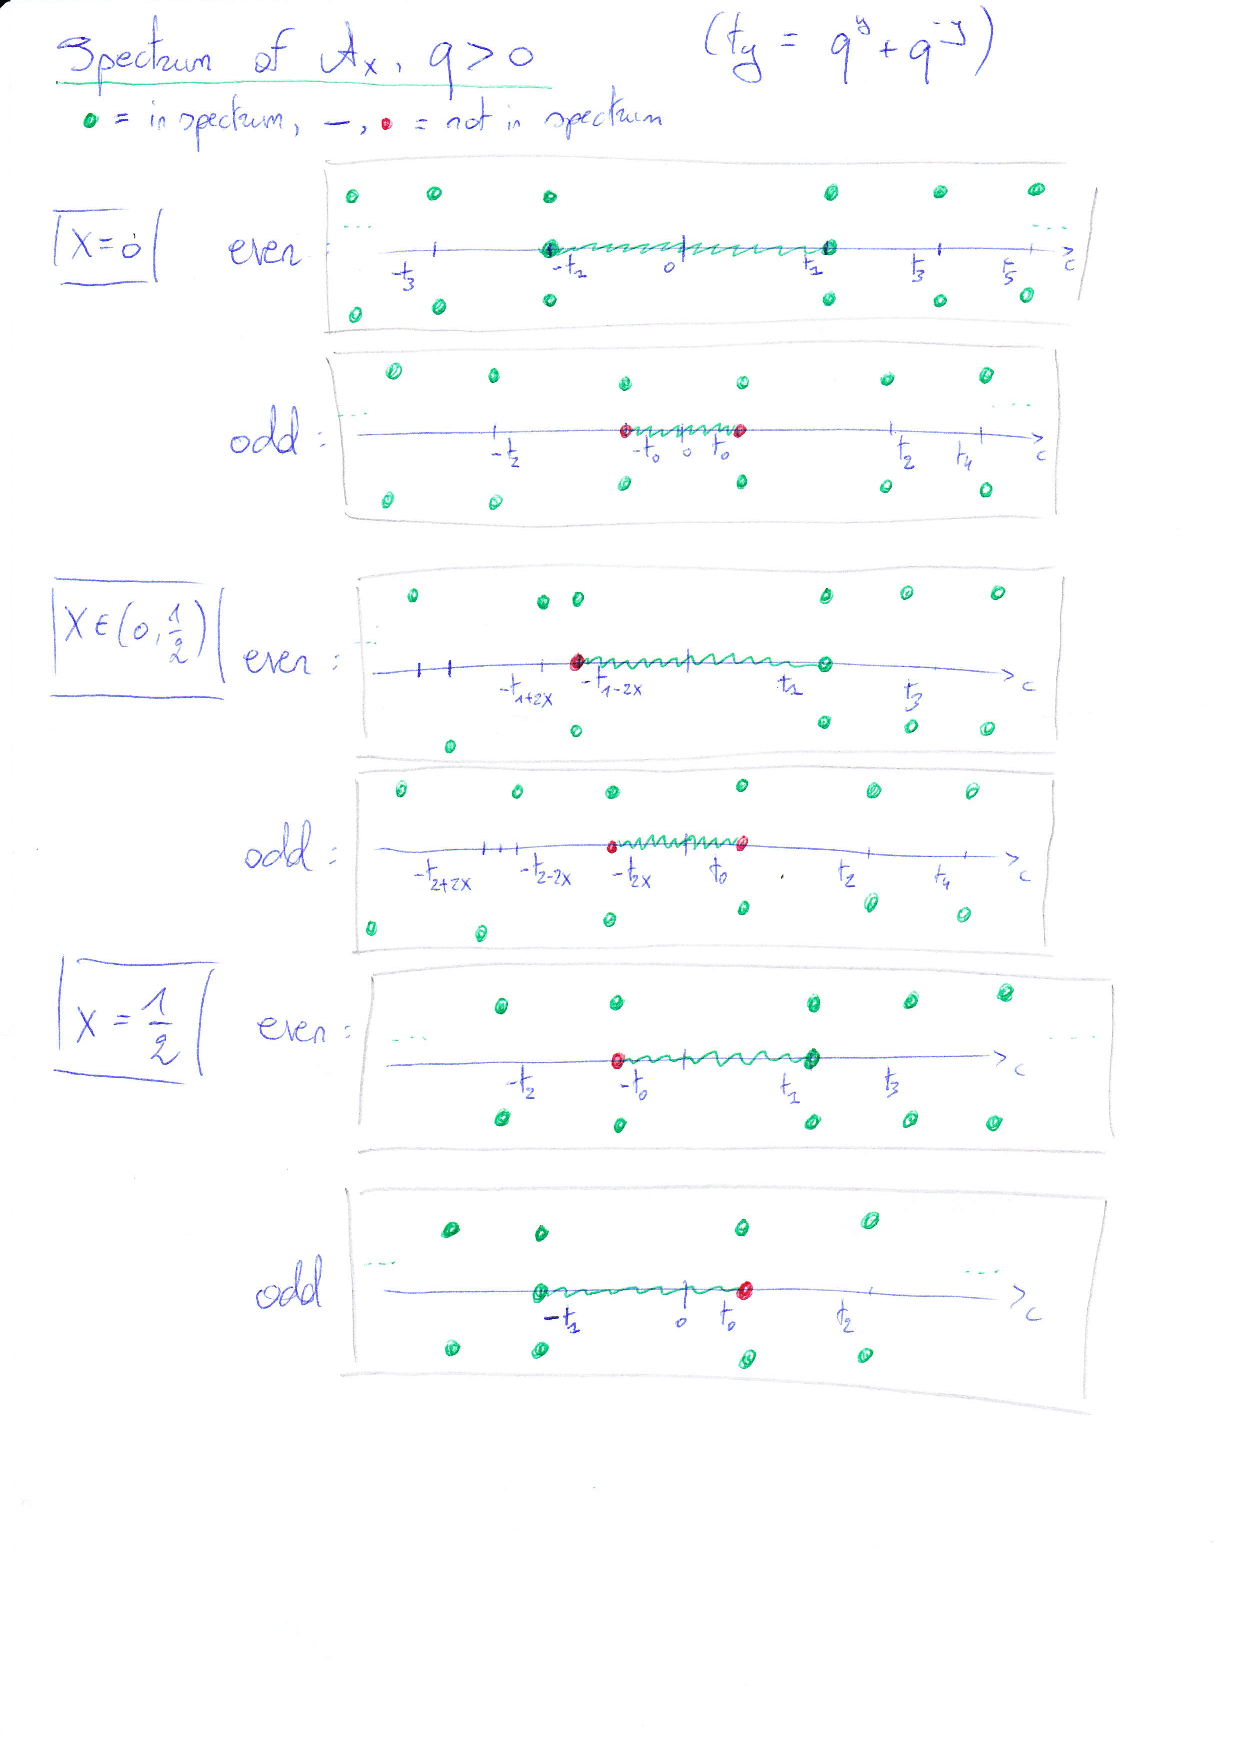
\includepdf[pages={1}]{ScanSpec.pdf}


% Make remark on regular representation cf. Koelink-Rosengren

% Include a concrete descripition of the universal envelope of $A_x$ from this?


%More generally, 

%As a concrete instance of the example of monoidal equivalence, let $\tilde{A}$ be the generalized compact Hopf face algebra obtained from the set $\tilde{I} =I_1\sqcup I_2$ with $I_1= \Z$ and $I_2= \{\bullet\}$ with the $B_{kl} =\emptyset$ and $E(k,l)$ for $k,l\neq \bullet$ as in section ..., with $B_{k,\bullet} = B_{\bullet,k}= \emptyset$, and $B_{\bullet,\bullet} = \{\pm\}$ with $E_{\bullet,\bullet} = \begin{pmatrix} 0 & |q|^{1/2} \\ -\sgn(q)|q|^{-1/2}&0\end{pmatrix}$ (with the basis ordered as $-,+$). Then this will be obtained from the direct sum of the functor from ... and the ordinary forgetful functor from $\Rep(SU_q(2))$ into $\Hilb$. It follows that the components $\tilde{A}(ij)$ can be described by the generators and relations as in ..., but with $F(\lambda)$ and $F(\rho)$ set equal to 1 whenever the corresponding index is $\bullet$.




% Study spectrum fundamental character
% Study dual quantum groupoid
% Make connection with dynamical cocycle
% In case of qgroupoid constructed from identity functor for Rep(SU_q(2)): rep theory of associated Galois object should just be: a single representation (Galois object is type I factor, cutdown of $B(\mathscr{L}^2(SU_q(2)))$). Yes: in general, Galois object is Morita equivalent with algebra of original ergodic action, should also be stressed for Podles spheres

\section{The reduced C$^*$-algebra of the dynamical quantum $SU(2)$ group}

We now study the reduced C$^*$-algebra $\mathcal{A}_x$ associated to $(\mathscr{A}_x,\Delta)$. It will be convenient here to use the linking partial compact quantum group between $\mathscr{A}(\Gamma_x)$ and $\Pol(SU_q(2))$.  Let us denote $\widetilde{\Gamma}_x = \Gamma_x\cup \{\bullet\}$, the disconnected sum of $\Gamma_x$ with the graph $\bullet$ consisting of a single vertex and two loops denoted $+$ and $-$ with respective weights $q$ and $q^{-1}$ and respective signs $+$ and $-\sigma$. Then the partial Hopf $^*$-algebra associated to the above-mentioned linking partial compact quantum group is $\mathscr{A}(\widetilde{\Gamma}_x)$. It splits into four components $\mathscr{A}(\Lambda,\Lambda')$, where $\Lambda,\Lambda' \in \{\Gamma_x,\Gamma\}$, and with the total algebras of these components generated by the $u_{e,f}$ with $e \in \Lambda,f\in \Lambda'$. We have $\mathscr{A}(\Gamma_x,\Gamma_x) = \mathscr{A}_x$ and $\mathscr{A}(\bullet,\bullet) = \Pol(SU_q(2))$. Let us investigate the remaining components.

In fact, the total algebra $A_{x,\bullet} = A(\Gamma_x,\bullet)$ was studied in \cite{DCY1}. Following the discussion in Section \cite{SecUni}, its generators can be written as \[(u_{\epsilon,\nu})_{q^{x+k}} =  u_{(k,k-\epsilon),\nu}, \qquad k\in \Z,\epsilon,\nu \in \{+,-\}\] the base algebra being reduced to a single copy of $\Fun_{\fin}(\Lambda_x)$ whose elements we write in the form $f(\lambda)$. The remaining disussion in Section \cite{SecUni} is then just as before, except that one now puts $w_+(\rho) = q, w_-(\rho) = q^{-1}$, i.e.~ the limit $\rho\rightarrow +\infty$ is taken. A similar discussion holds for $A_{\bullet,x} = A(\bullet,\Gamma_x)$, with the roles of $\rho$ and $\lambda$ interchanged. 

Now the total comultiplication of $A(\widetilde{\Gamma}_x)$ splits into parts \[\Delta_{\Lambda,\Lambda''}^{\Lambda'}: A(\Lambda,\Lambda'')\rightarrow M(A(\Lambda,\Lambda')\otimes A(\Lambda',\Lambda'')),\quad \Lambda,\Lambda',\Lambda'' \in \{\Gamma_x,\bullet\}.\] Consider the invariant positive integral $\phi$ on $A(\widetilde{\Gamma}_x)$. Then by invariance, we have \[\phi(a) = (\phi\otimes \phi)(\Delta_{\Gamma_x,\Gamma_x}^{\bullet}(a)),\qquad a \in A(\Gamma_x).\] It follows that the reduced C$^*$-algebra of $\mathcal{A}(\Gamma_x)$ can be understood as the completion of $\Delta_{\Gamma_x,\Gamma_x}^{\bullet}(A(\Gamma_x))$ in $\mathcal{A}_{x,\bullet}\otimes \mathcal{A}_{\bullet,x}$. 

Let us thus first study the reduced C$^*$-algebraic completion $\mathcal{A}_{x,\bullet}$. Note that $\phi$ is supported on $\sum_y \lambda_y A_{x,\bullet}\lambda_y$. Now any element of $A_{x,\bullet}$ can be written as linear combination of a polynomial in the $\alpha,\beta,\gamma,\delta$ times a finite support function on $\Lambda_x$. It easily follows then that $\lambda_y A_{x,\bullet}\lambda_y$ is generated by $\beta^*\beta\lambda_y,\alpha\beta^*\lambda_y$ and $\beta\alpha^*\lambda_y$. Let us fix $y$, and write \begin{eqnarray*} X_y &=& \ctau(y/q)\alpha \beta^*\lambda_y,\\ qZ_y &=& (y^{-1}-\ctau(y)\beta^*\beta)\lambda_y\\ Y_y &=& \ctau(y/q)\beta \alpha^*\lambda_y.\end{eqnarray*}  Then using that formally $Z_y = \lim_{\rho\rightarrow +\infty} \rho^{-1}\Omega \lambda_y$, we find that $X_yZ_y = q^2Z_yX_y$, $Y_yZ_y= q^{-2}Z_yY_y$, $Z_y^*=Z_y$ and \begin{eqnarray*} X_yY_y &=& 1+ q (y^{-1}-y)Z_y -  q^2 Z_y^2 \\ Y_yX_y &=& 1+ q^{-1}(y^{-1}-y)Z_y-q^{-2}Z_y^2,
\end{eqnarray*}
where we have treated $\lambda_y$ as the unit of $\lambda_y A_{x,\bullet}\lambda_y$.

We see that we obtain a copy of a (non-standard) Podle\'{s} sphere $\mathbb{S}_{q,y}^2$. Moreover, $\Delta_{x,\bullet}^{\bullet}$ restricts to the ordinary action $SU_q(2)$ on this Podle\'{s} sphere. The associated C$^*$-algebra $C(\mathbb{S}_{q,y}^2)$ is then faithfully represented on $l^2(J_{y})$, where $J_y = q^{1+2\mathbb{N}}/y\cup -q^{2\mathbb{N}+1}y$, by $Z_ye_z = z e_{z}$ and \begin{eqnarray*} X_ye_{z} &=& \sigma_{qy} \lbrack (1-yz/q)(1+z/qy)\rbrack^{1/2}e_{q^{-2}z}\\ Y_ye_{z} &=& \sigma_{qy} \lbrack (1-qyz)(1+qz/y)\rbrack^{1/2}e_{q^2z}.\end{eqnarray*} The invariant state on the Podle\'{s} sphere is implemented by the (normalized) trace class operator associated to $|Z|$. 

Let us extend the above Podle\'{s} sphere representation to $A_{x,\bullet}$.  Let $J =\{(z,y)\mid y \in \Lambda_x, qz \in J_{y}\}$. Then we define the following representation of $A_{x,\bullet}$ on $l^2(J)$: \begin{eqnarray*} \alpha e_{y,z} &=&  \left(\frac{y+z/q}{\ctau(y)}\right)^{1/2}e_{qy,z/q}\\ \beta e_{y,z} &=&  \sigma_y \left( \frac{1/y-qz}{\ctau(y)}\right)^{1/2}e_{qy,qz},  \\  \alpha^* e_{y,z} &=&  \left(\frac{y/q+z}{\ctau(y/q)}\right)^{1/2}e_{y/q,qz} \\ \beta^* e_{y,z} &=& \sigma_{qy}\left( \frac{q/y-z}{\ctau(y/q)}\right)^{1/2}e_{y/q,z/q}
 \\ \lambda_{y'} e_{y,z} &=& \delta_{y,y'}e_{y,z}. \end{eqnarray*} It is easily seen that this is well-defined, that we get our standard representation on the $e_{z} = e_{qy,qz}$ for the Podle\'{s} sphere $\lambda_y A_{x,\bullet}\lambda_y$, and that this defines a $^*$-representation of $A_{x,\bullet}$. It is also easy to see this representation as a limit of the representations obtained in ...

% Reference to Zinn-Justin Banica paper

It is now easy to find also a $^*$-representation of $A_{\bullet,x}$. Here the relations between the generators are obtained from $A_{x}$ by letting $\lambda\rightarrow +\infty$. In fact we have \[S^2(u_{\epsilon,\nu}) = \frac{w_{\epsilon}(\lambda)}{w_{\nu}(\rho)} u_{\epsilon,\nu},\] hence the unitary antipode $R$ satisfies \[ R(u_{\epsilon,\nu}) = u_{\nu,\epsilon}^* \frac{w_{\nu}^{1/2}(\lambda)}{w_{\epsilon}^{1/2}(\rho)}\] By composing with $*$ and the obvious conjugacy operator, it follows that we have a $^*$-algebra isomorphism \[u_{\epsilon,\nu} \mapsto  \frac{w_{\nu}^{1/2}(\lambda)}{w_{\epsilon}^{1/2}(\rho)}u_{\nu,\epsilon},\] which as well gives an identification $A_{\bullet,x}\rightarrow A_{x,\bullet}$. Concretely, this gives \[\alpha \mapsto q^{1/2}w_{-}^{1/2}(\lambda) \alpha,\qquad \beta \mapsto -\sigma\beta^*.\] Hence, for $A_{\bullet,x}$ we obtain the $^*$-representation on $l^2(J_{y})$ by \begin{eqnarray*} \alpha e_{y,z} &=&  \left(\frac{qy+z}{\ctau(qy)}\right)^{1/2}e_{qy,z/q}\\ \beta e_{y,z} &=&  - \sigma_{y} \left( \frac{q/y-z}{\ctau(y/q)}\right)^{1/2}e_{y/q,z/q}\\ \rho_{y'}e_{y,z} &=& \delta_{y',y}e_{y,z}.\end{eqnarray*}

Finally, let us consider then the $^*$-representation of $A_{x}$ on $l^2(J)\boxtimes l^2(J)$, which is just $l^2(J)\otimes l^2(J)$. Let us identify the basis of the latter by $e_{y,z,y',z'} = e_{y,z}\otimes e_{y',z'}$. Then \begin{eqnarray*} \alpha e_{y,z,y',z'} &=& \left(\frac{(y+z/q)(qy'+z')}{\tau(y)\tau(qy')}\right)^{1/2}e_{qy,z/q,qy',z'/q}  \\ && \qquad + \left(\frac{(1/y-qz)(1/qy' -z')}{\tau(y)\tau(qy')}\right)^{1/2}e_{qy,qz,qy',qz'}, \\
\beta e_{y,z,y',z'} &=&  \sigma_y \left(\frac{(1/qy-z)(y'+qz')}{\tau(y)\tau(y'/q)}\right)^{1/2}e_{qy,qz,y'/q,qz'}  \\ &&\qquad -\sigma_{y'}\left(\frac{(y+z/q)(q/y'-z')}{\tau(y)\tau(y'/q)}\right)^{1/2} e_{qy,z/q,y'/q,z'/q}
\end{eqnarray*}

We see that there is an obvious observable in the commutant, namely the quantity $z/z'$. 

Fix now $y,y'$, and write $e_{z,z'} = e_{y,z,y',z'}$. Then writing $\tilde{\Omega} =  \sigma_y\sigma_y'\tau(y)\tau(y'/q) \Omega$, we have \begin{eqnarray*}  \tilde{\Omega} e_{z,z'} &=& \lbrack (1/qy-z)(y'+qz')(y+qz)(q/y'-q^2z')\rbrack^{1/2} e_{q^2z,q^2z'} \\ && + \sigma_{yy'} \left(\tau(qy/y')\tau(y)\tau(y'/q) - (1/qy-z)(y'+qz') - (y+z/q)(q/y'-z')\right) e_{z,z'} \\ && + \lbrack (1/qy-z/q^2)(y'+z'/q)(y+z/q)(q/y'-z')\rbrack^{1/2} e_{q^{-2}z,q^{-2}z'}
\end{eqnarray*}



%%% Local Variables: 
%%% mode: latex
%%% TeX-master: "dyn-suq-main"
%%% End: 
